%17/02 - Aythami Morales 
\chapter{Aprendizaje no supervisado - Clustering}
\section{Clustering}
En el aprendizaje supervisado, obtenemos el valor de y que nos permite medir el rendimiento. Así, todo el algoritmo está pensado en explotar y. En el aprendizaje no supervisado, solo tenemos datos y no las etiquetas asociadas. Esto sirve para obtener un conocimiento, el cual se puede obtener mediante un agrupamiento de los datos en función de unas características o similitudes. A esto se le conoce como clustering. 

El clustering se basa en la proximidad entre datos o ítems. Proximidad puede hacer referencia a la distancia euclídea (la distancia más corta) entre los dos puntos, pero no es la única forma de medir similitud. Por ejemplo, en datos binarios, se puede medir la distancia euclídea, pero lo más natural es utilizar una distancia hamil, que mira el promedio de bits que varían. Otras distancias son la distancia de Manhattan, donde solo podemos desplazarnos de forma horizontal o vertical (no en diagonal). 

Medir la proximidad en palabras es complicado, pero es lo que hacen los LMMs. Su complejidad radica en la importancia social y cultural de las palabras. 

En el caso de las distribuciones estadísticas, hay una familia de distancias que permiten averiguar esos datos. El resumen de todo esto es que la proximidad es más compleja de lo que puede parecer, y se debe ajustar a los datos que tengamos. 

En clustering, dados unos datos, se pueden asignar a los clústeres definidos en función de la proximidad. Se asignan datos nuevos a un clúster, pero no hay que confundirlo con clasificación. Mientras que clustering es aprendizaje no supervisado, la clasificación sí lo es, ya que se utilizan las etiquetas de los datos para, a datos nuevos, asignarles esas etiquetas.

El análisis de cluster se puede definir como la organización de una «colección de patrones en clústers basados en la similitud» (Jain, Murty, et al. 1999).
La definición y el alcance de «cluster» en el conjunto de datos no son fáciles de definir. Según (Jain y Dubes 1988), un cluster es:
\begin{itemize}
\item conjunto de objetos similares
\item conjunto de puntos en un clúster en el entorno de prueba / la distancia entre dos puntos de un clúster es menor que la distancia entre cualquier punto del clúster y cualquier punto de otros clústers
\item regiones densamente conectadas en un espacio multidimensional separadas por puntos poco conectados
\end{itemize}

\subsection{Distancia}
La distancia entre dos instancias $x^{(i)}$ y $x^{(j)}$, que es una distancia métrica, mide si satisface las siguientes propiedades:
$$d(\vec{x}^{(i)}, \vec{x}^{(j)}) \leq d(\vec{x}^{(i)}, \vec{x}^{(k)}) + d(\vec{x}^{(k)}, \vec{x}^{(j)}), \forall  \vec{x}^{(i)}, \vec{x}^{(j)}, \vec{x}^{(k)} \in \mathbb{R}^n$$

$$d(\vec{x}^{(i)}, \vec{x}^{(j)}) = 0 \rightarrow \vec{x}^{(i)} = \vec{x}^{(j)}, \forall \vec{x}^{(i)}, \vec{x}^{(j)} \in \mathbb{R}^n$$

\section{Algoritmo K-means}
K-means es el algoritmo típico de aprendizaje no supervisado de clústering. Tenemos unos valores no etiquetados. El primer paso es elegir el número de clústeres que se quieren, y se inicializan aleatoriamente dos centroides, es decir, puntos que sirven para el aprendizaje. 

El primer paso es calcular la distancia de cada punto al centroide y asignar el dato al centroide más cercano (con distancia menor). El segundo paso es la actualización del centroide, moverlo a la ubicación media de los puntos, como si fuera un centro de masas o centro geométrico. Tras esto, se vuelve al paso 1 y se reasignan los datos a los nuevos centroides. Así, estos dos pasos se repiten hasta que los centroides no cambien.

Para definir el algoritmo, la entrada son el número de clústeres K y unos datos de entrenamiento. Se inicializan K centroides de forma aleatoria y se repiten de forma iterativa los pasos de asignación de datos a un clúster y recalcular las coordenadas de cada centroide. 

\begin{figure}[h]
\centering
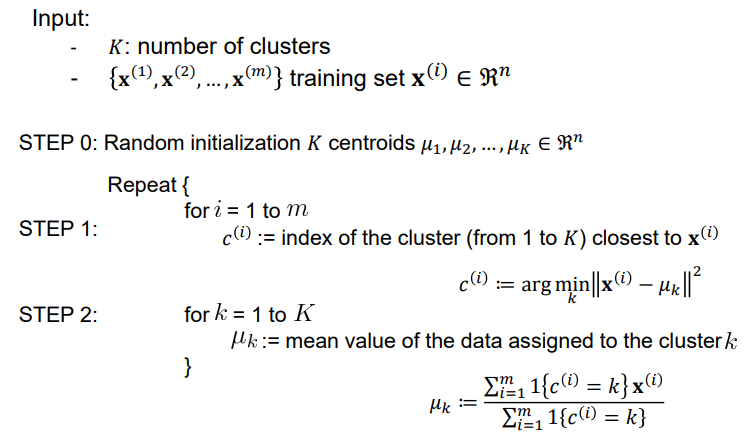
\includegraphics[width = 0.8\textwidth]{figs/kmeans-algorithm.png}
\end{figure}

\subsection{Superposición entre clústeres}
Cuando los clústeres se superponen, se habla de clústeres difusos. Un ejemplo es con las tallas de ropa S, M y L. La diferencia entre S y L está clara, pero hay algunos puntos que están en una frontera difusa y puede pertenecer a uno u otro clúster.

\subsection{Inicialización aleatoria y óptimos}
Una solución para la inicialización aleatoria es coger dos datos al azar y asignar el centroide inicialmente a esos datos, para asegurar estar en rango. Al hacer esto, el algoritmo no es determinista, ya que los resultados no van a ser siempre los mismos, aunque pueda haber resultados más y menos estables. 

Cuando no hay tanta separación entre los datos, se pueden dar soluciones dispares. Esto se puede resolver mediante la repetición y medir el rendimiento de las distintas ejecuciones para ver qué solución es la mejor. Se calcula la distancia de cada punto a su centroide y la solución que minimice esa distancia es la que obtiene los centroides más óptimos. 